
\documentclass[10pt]{article}



\usepackage{sectsty}
\chapternumberfont{\Large}
\chaptertitlefont{\Large}
\usepackage{graphicx}
\usepackage{eso-pic}
\usepackage{subfigure}
\usepackage{subcaption}
\usepackage{booktabs}% http://ctan.org/pkg/booktabs
\newcommand{\tabitem}{~~\llap{\textbullet}~~}
\usepackage[english]{babel}
\usepackage[utf8]{inputenc}
\usepackage[T1]{fontenc}
\usepackage{fancyhdr}
\usepackage{float}
\usepackage[justification=centering]{subfig}
\usepackage[margin = 0.8in]{geometry}
\usepackage{titlesec} % Control title sizes
\usepackage{multirow}
\usepackage{mathtools}
\usepackage{setspace}
\usepackage{wrapfig}
\usepackage{yfonts}
\usepackage{url}
\usepackage{placeins}

\usepackage{amsmath}
\usepackage{amssymb}
\DeclareMathOperator{\Tr}{Tr}
\usepackage{gensymb}
\usepackage{emptypage}
\usepackage{lastpage}
\usepackage[colorlinks = true, linkcolor = blue]{hyperref}
\numberwithin{equation}{section}
\numberwithin{figure}{section}
\numberwithin{table}{section}
\usepackage{caption}
\usepackage{wrapfig}
\usepackage{tikz} % For drawing figures
\usepackage{verbatim} % Making comment section
\usepackage{dirtytalk}
\usepackage[demo]{graphicx}

\usepackage{subcaption}
\usepackage{indentfirst}

\begin{titlepage}
\thispagestyle{empty}
\end{titlepage}

\begin{document}

\begin{center}

\begin{center}
%\includegraphics[scale=0.5]{fig/windmill.PNG}

\includegraphics[height=4cm]{Figures/dtulogo.jpg}
\end{center}
\vspace*{1.8cm}
\newcommand{\HRule}{\rule{\textwidth}{1mm}}
\HRule\\
[0cm]\fontsize{14}{16}{\textbf{Machine Learning and Data Mining Report 1 \linebreak Algerian Forest Fires}} \linebreak 
\fontsize{16}{32}{\textbf{\\[10pt] }}
\HRule\\[0.5cm]
\renewcommand{\arraystretch}{1}
\vspace*{0.5cm}
\Large{
\vspace*{0.5cm}

\begin{tabular}{l l l l}
\large{Student no.:{\ \ s192322\ }} & \large{Student:{\ \ Paolo Dalpasso\ \ \ \ \ \ \ \ \ }}\\
\large{Student no.:{\ \ s206063\ }} & \large{Student:{\ \ Changzhi Ai\ \ \ \ \ \ \ \ \ }}\\
\large{Student no.:{\ \ s192624\ }} & \large{Student:{\ \ Boris Guillerey\ \ \ \ \ \ \ \ \ }}\\
\vspace{1cm}
\end{tabular}\\ 

\end{center}

\setlength{\parindent}{5ex}

\pagebreak

\tableofcontents

\pagebreak

% \section*{Contributions}
%  The group split the work amongst themselves as is depicted in \autoref{table:contributions}.

% \begin{table}[H]
% \centering
% \begin{tabular}{l|c|c|c|}
% \cline{2-4}
%                                                                                & \textbf{Changzhi} & \textbf{Paolo} & \textbf{Boris} \\ \hline
% \multicolumn{1}{|l|}{\textbf{Data set description}}                            & X                 & X              &                \\ \hline
% \multicolumn{1}{|l|}{\textbf{Data attributes explanation}}                     &                   & X              & X              \\ \hline
% \multicolumn{1}{|l|}{\textbf{Outliers}}                                        &                   &                & X              \\ \hline
% \multicolumn{1}{|l|}{\textbf{Regional comparison}}                             &                   & X              &                \\ \hline
% \multicolumn{1}{|l|}{\textbf{Similarity}}                                      & X                 & X              &                \\ \hline
% \multicolumn{1}{|l|}{\textbf{Correlation matrix}}                              & X                 &                & X              \\ \hline
% \multicolumn{1}{|l|}{\textbf{Classification from given meteorological inputs}} &                   &     X           & X              \\ \hline
% \multicolumn{1}{|l|}{\textbf{Principal component analysis}}                    &                   & X              & X              \\ \hline
% \multicolumn{1}{|l|}{\textbf{Perspective of Machine Learning study}}           &   X                &                & X              \\ \hline
% \end{tabular}
% \caption{Group's contribution table.}
% \label{table:contributions}
% \end{table}


\section{Data set description}
\subsection{Data explanation}
The data set contains two groups of data of two regions of Algeria: the Sidi Bel Abbès region located in the northwest of Algeria and the Bejaia region located in the northeast of Algeria (see \autoref{fig:map}).

\begin{figure}[H]
    \centering
    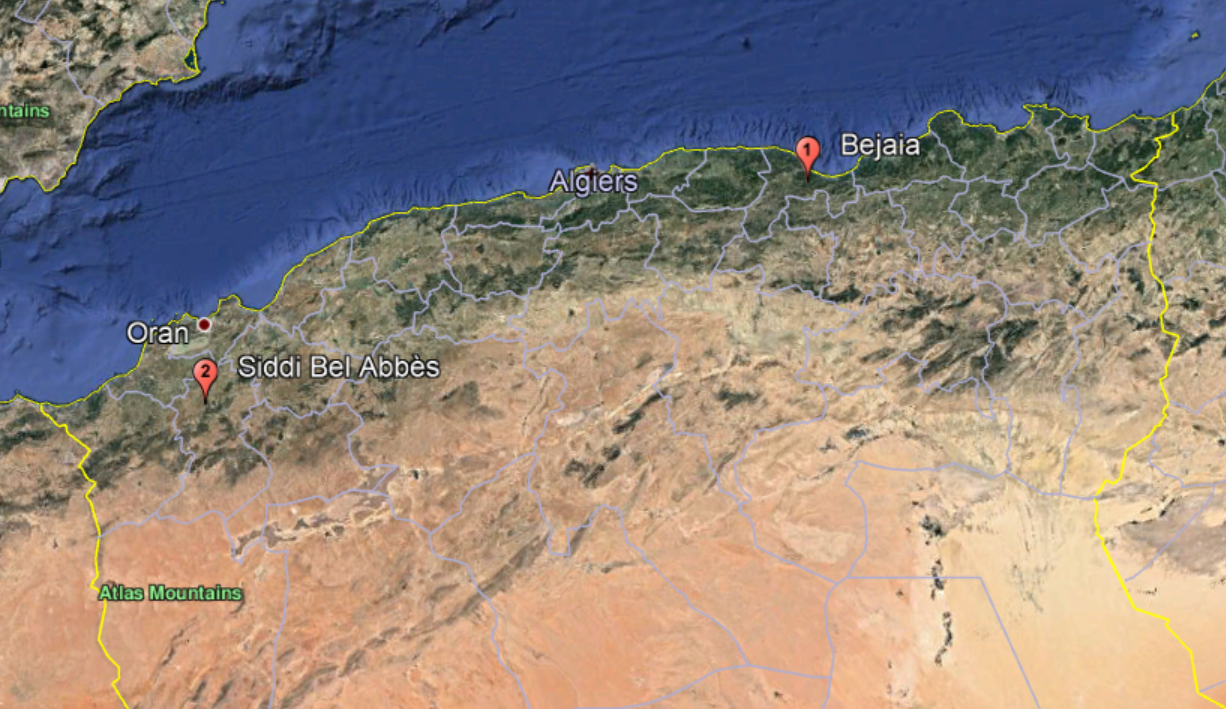
\includegraphics[scale=0.6]{Figures/Algeria_map.png}
    \caption{Map of Northern Algeria with the two regions considered in the study (Google Earth).}
    \label{fig:map}
\end{figure}


The used dataset includes 244 instances (122 for each region). The data were collected daily between June and September 2012, since the fire occur more frequently in the summer period. The dataset contains meteorological data and indexes from the Fire Weather Index system.


\subsection{Data source}
The data is provided in the online Machine Learning Repository of Center for Machine Learning and Intelligent Systems of UCI. (\url{https://archive.ics.uci.edu/ml/datasets/
Algerian+Forest+Fires+Dataset++})

\subsection{Summary of previous work on the dataset}
The dataset was previously used by researchers Faroudja Abid and Nouma Izeboudjen. The objective of the two researchers was to use data mining to create an algorithm capable of predicting and notify the appearance of wild forest fires, without the necessity of human monitoring. The algorithm was based on a Decision Tree (DT) and implemented in a sensor node system. Meteorological data, such as relative humidity and temperature, as well as Fire Weather Indexes collected from 2 different regions of Algeria, Bejaia and Sidi-Bel Abbès, were used to train the decision tree algorithm.\cite{article}

\subsection{Data classification and regression}
Classification and regression will be performed on the data as part of the second project of the course. Classification would be employed to predict the ignition of fires and regression to determine the Fire Weather Index. More about the perspectives of ML algorithms is described in \autoref{Perspectives}. 


\section{Data attributes explanation}

\subsection{Definitions and types  of attributes}
The dataset contains 12 attributes which can be classified in tow categories: meteorological attributes and indices from the FWI system. They are provided in the following order:

\begin{itemize}
    \item \textbf{Date (Discrete, Interval):\\} The day (DD/MM/YYYY) when the measurements were conducted, from June 2012 to August 2012. 
    
    \item \textbf{Temperature (Discrete, Interval):\\} Temperature at noon ( temperature max) in Celsius degrees.
    
    \item \textbf{Relative humidity (Discrete, Ratio):\\} The ratio of the actual water vapour pressure to the saturation water vapour pressure in percentage.
    
    \item \textbf{Wind speed (Discrete, Ratio):\\} Wind speed in km/h.
    \item \textbf{Rain (Continuous, Ratio):\\} Daily amount of precipitation in mm\textbackslash m$^2$.
    
    \item \textbf{Fine Fuel Moisture Code (Continuous, Ratio):\\} It represents fuel moisture of forest litter fuels under the shade of a forest canopy, the equivalent of 16-hour timelag.
    
    \item \textbf{Duff Moisture Code (Continuous, Ratio):\\}
    It represents fuel moisture of decomposed organic material underneath the litter.
    \item \textbf{Drought Code (Continuous, Ratio):\\}
    It represents drying deep into the soil.
    
    \item \textbf{Initial Spread Index (Continuous, Ratio):\\}
    It estimates the spread potential of the fire.
    
    \item \textbf{Buildup Index (Continuous, Ratio):\\}
    It estimate the potential heat released by the fire in heavier fuels.
    
    \item \textbf{Fire Weather Index (Continuous, Ratio):\\}
    It represent the general fire intensity potential.
    
    \item \textbf{Fire \textbackslash Not Fire (Binary):\\}
    It indicates if a fire has been spotted or not during the day.
    
\end{itemize}

It is worth stressing that the indices, from FFMC to FWI are part of the more general calculation of the Fire Weather Index system. An online calculator can be found here: \url{https://fire.synopticlabs.org/tools/fwi/}. This calculation model is also called the Canadian Forest Weather Index, as it had been developed and enforced in Canada in the 1970s. The fourth version of the model, the one currently in use, has been developed by C.E. Van Wagner in 1987. A detailed description of the model, including the calculations can be found in \cite{FWI_Wagner}. The general structure is presented in \autoref{fig:FWIstructure}

\begin{figure}[H]
    \centering
    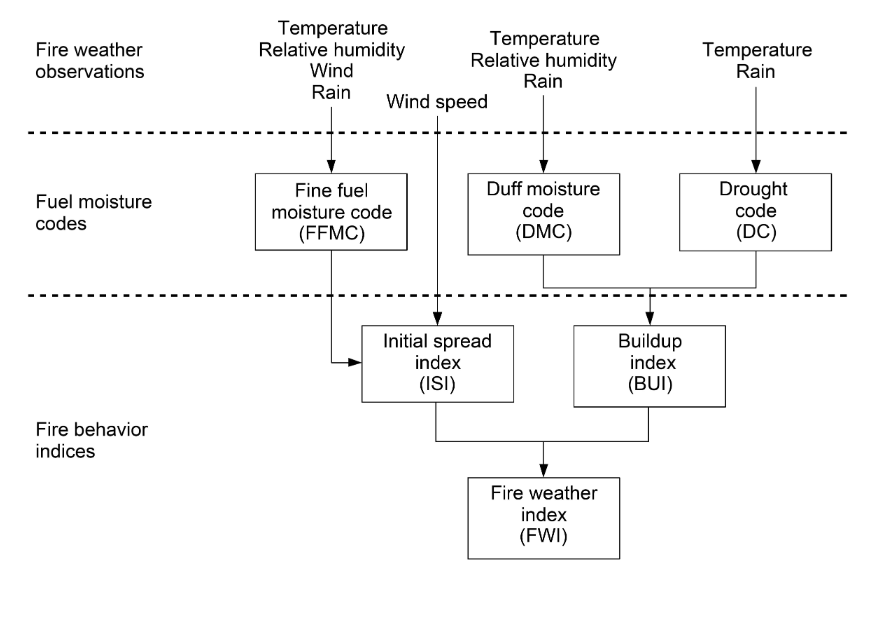
\includegraphics[scale=0.8]{Figures/FWI_structure.png}
    \caption{Structure of the FWI system (source: Van Wagner 1987 \cite{FWI_Wagner})}
    \label{fig:FWIstructure}
\end{figure}

\subsection{Data issues}
One observation has its attributes shifted in the csv file. This has been corrected directly in this file.

\section{Data visualization}
\label{section:data visualisation}
\subsection{Outliers}

Each attribute was analysed independently via histograms (see e.g. \autoref{fig:TempBejaia}) and boxplots (see \autoref{boxplot_data}) in order to detect possible outliers. This investigation did not evidence any outliers in the data. We especially do not consider the highest values of precipitations as outliers because it is expected some rare extreme events which should be accounted in the studied case.  

\begin{figure}[H]
    \centering
    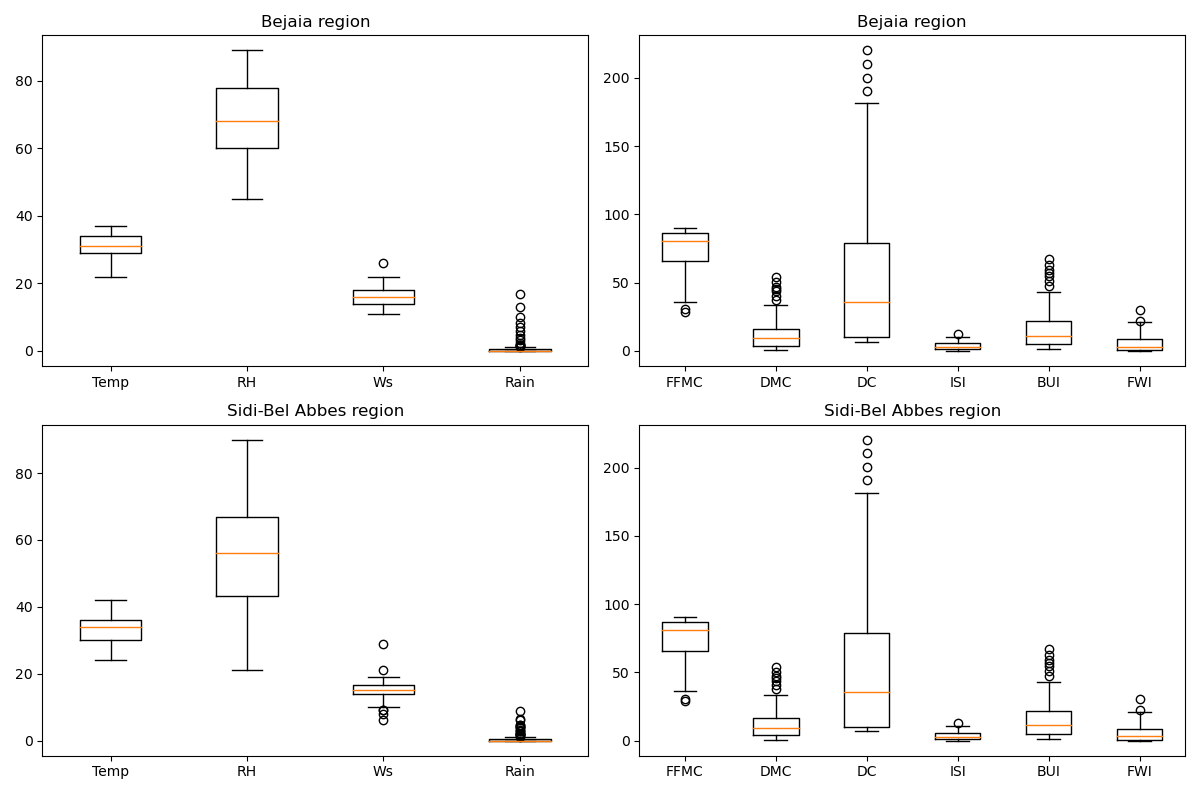
\includegraphics[width=\textwidth,height=\textheight,keepaspectratio]{Figures/boxplot_data.png}
    \caption{Boxplot of the attributes for both regions}
    \label{boxplot_data}
\end{figure}

\begin{figure} [H]
    \centering
    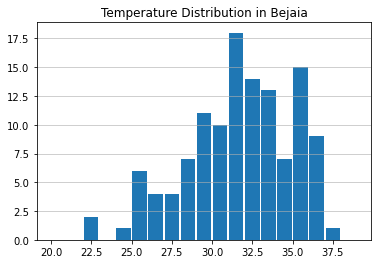
\includegraphics[scale=0.65]{Figures/Temp_Bejaia.png}
    \caption{Distribution of the temperature in the region of Bejaia in °C.}
    \label{fig:TempBejaia}
\end{figure}

\subsection{Regional comparison}
\label{section:data visualisation}
\begin{table}[H]
\centering
\begin{tabular}{|l|c|c|c|c|}
\hline
\textbf{Attribute}              & \textbf{Average} & \textbf{Standard Deviation} &\textbf{Median} &\textbf{Range}   \\ \hline
\textbf{Temp (°C)}              & 31.2                       & 3.32              & 31.0     & 15.0             \\ \hline
\textbf{Relative humidity (\%)} & 68.0                       & 11.15             & 68.0     & 44.0               \\ \hline
\textbf{Wind speed (km/h)}      & 16.0                       & 2.84              & 16.0     & 15.0              \\ \hline
\textbf{Rain (mm/day)}          & 0.84                       & 2.40              & 0.0      &  16.8              \\ \hline
\textbf{FFMC}                   & 74.7                       & 15.55             & 80.9     &  61.69              \\ \hline
\textbf{DMC}                    & 12.3                       & 11.27             & 9.45     & 53.5               \\ \hline
\textbf{DC}                     & 53.2                       & 51.77             & 35.55    & 213.5                \\ \hline
\textbf{ISI}                    & 3.7                        & 3.021             & 2.65     & 12.5               \\ \hline
\textbf{BUI}                    & 15.4                       & 14.47             & 11.2     & 66.30               \\ \hline
\textbf{FWI}                    & 5.6                        & 6.34              & 3.0      & 30.2             \\ \hline
\end{tabular}
\caption{Statistics of the 10 attributes in Bejaia Region}
\label{table:statistics_bejaia}
\end{table}


\begin{table}[H]
\centering
\begin{tabular}{|l|c|c|c|c|}
\hline
\textbf{Attribute}              & \textbf{Average} & \textbf{Standard Deviation} &\textbf{Median} &\textbf{Range}   \\ \hline
\textbf{Temp (°C)}              &    33.1                    &    3.67           & 34.0     &  18.0            \\ \hline
\textbf{Relative humidity (\%)} &   55.90                     &       15.71       &    56.0  & 69.0               \\ \hline
\textbf{Wind speed (km/h)}      &   15.0                     &      2.69         & 15.0     &   23.0            \\ \hline
\textbf{Rain (mm/day)}          &   0.67                     &      1.48         & 0.0      &   8.7            \\ \hline
\textbf{FFMC}                   &   81.10                     &      12.24        & 84.85     & 58.1             \\ \hline
\textbf{DMC}                    &   17.03                     &      12.99        &  13.15    &  65.0             \\ \hline
\textbf{DC}                     &   45.41                     &      42.92        &  31.5   & 170.0               \\ \hline
\textbf{ISI}                    &   5.89                      &       4.83       &   4.6   &  18.9              \\ \hline
\textbf{BUI}                    &    17.90                    &       13.87       &  13.89    &  66.6              \\ \hline
\textbf{FWI}                    &   8.80                      &       8.78        &  6.05     &   31.1          \\ \hline
\end{tabular}
\caption{Statistics of the 10 attributes in Sidi-Bel Abbès Region}
\label{table:statistic_Sidi}
\end{table}
The occurrence of fires was 48.3\% in Bejaia and 64.7\% in Sidi-Bel Abbes. A first inspection of the data (see \autoref{table:statistic_Sidi} and \autoref{table:statistics_bejaia}) shows that the higher frequency of fires in Sidi-Bel Abbes seems to be associated with higher temperature, lower relative humidity and lower precipitations. Overall, a more arid climate is observe in Sidi-bel Abbès, which seems to stimulate the emergence of fires.

\subsection{Similarity}

\indent The similarity between the attributes of the two regions is calculated using the cosine similarity: 

\begin{equation}
    cos(x,y) =  \frac{x^{T}y}{\|x\|\|y\|}
\end{equation}

\noindent Cosine similarity measures the similarity between two vectors by taking the
cosine of the angle the two vectors make in their dot product space. If the angle is
zero, their similarity is one, the larger the angle is, the smaller their similarity.

The result are shown in table \autoref{table:similarity}:


\begin{table}[H]
\centering
\begin{tabular}{|l|c|c|}
\hline
\textbf{Attribute for both regions}              & \textbf{Cosine Similarity} & \textbf{Extended Jaccard Similarity} \\ \hline
\textbf{Temp (°C)}              & 0.9969      &         0.9901                     \\ \hline
\textbf{Relative humidity (\%)} & 0.9651      &         0.9069                  \\ \hline
\textbf{Wind speed (km/h)}      & 0.9688      &          0.9358                   \\ \hline
\textbf{Rain (mm/day)}          & 0.1060      &            0.0506                \\ \hline
\textbf{FFMC}                   & 0.9814      &           0.9585                 \\ \hline
\textbf{DMC}                    & 0.8957      &             0.7676                 \\ \hline
\textbf{DC}                     & 0.8772      &            0.7612                  \\ \hline
\textbf{ISI}                    & 0.7276      &            0.4891                   \\ \hline
\textbf{BUI}                    & 0.8917      &             0.8010                  \\ \hline
\textbf{FWI}                    & 0.6902      &             0.5239                 \\ \hline
\end{tabular}
\caption{Similarity between attributes from both regions}
\label{table:similarity}
\end{table}

Observing the table, we can notice that the attributes that change the most between the 2 regions are the precipitation of rain per day and the FWI (Fire Weather Index). Both the data are on average higher in the Sidi-Bel Abbès region, which could explain the higher presence of forest fires.


A heat map of the Cosine similarity for all 10 attributes of both regions is displayed in \autoref{fig:CosineSimilarity}. It can be seen that there are strong relations between relative humidity and temperature, wind speed and temperature, wind speed and relative humidity, FFMC and temperature, FFMC and relative humidity, FFMC and wind speed.
\begin{figure} [H]
    \centering
    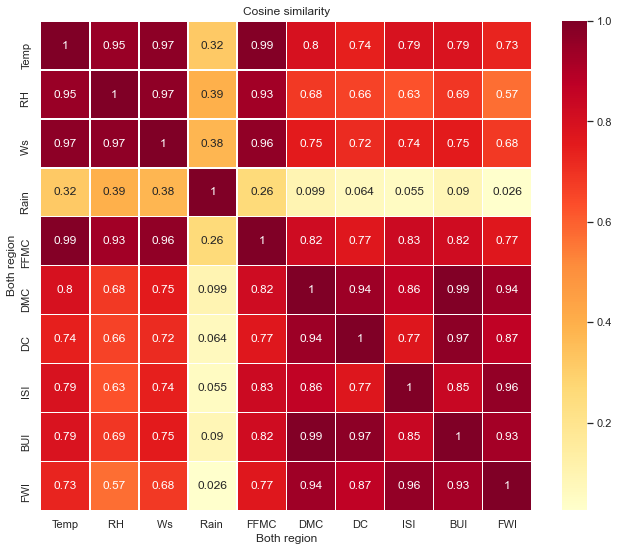
\includegraphics[scale=0.50]{Figures/CosineSimilarity.png}
    \caption{Heat map of the Cosine similarity for all 10 attributes of the both region studycase.}
    \label{fig:CosineSimilarity}
\end{figure}

\subsection{Correlation matrix}
\label{correlationStudy}

The correlation matrix is calculated via the following formula:

\begin{equation}
    cor[x_i,x_j]=\frac{cov[x_i,y_j]}{s_is_j}
\end{equation}

\noindent where $s_i$ and $s_j$ are the standard deviations of attributes $i$ and $j$ respectively. On \autoref{fig:heatmap} the correlation coefficients are reproduced between each attribute. Especially, we note a general positive correlation between all the indices derived from the FWI system (FFMC to FWI). All those parameters characterize, through different aspects, the tendency to fires ignition, so that their positive correlation is expected. The temperature and relative humidity are respectively positively and negatively correlated with all those indices. The rain, although in less measure, is also negatively correlated with the indices. Finally, the wind speed is not correlated with those indices but is slightly positively correlated with rain and relative humidity while negatively correlated with temperature.

\begin{figure} [H]
    \centering
    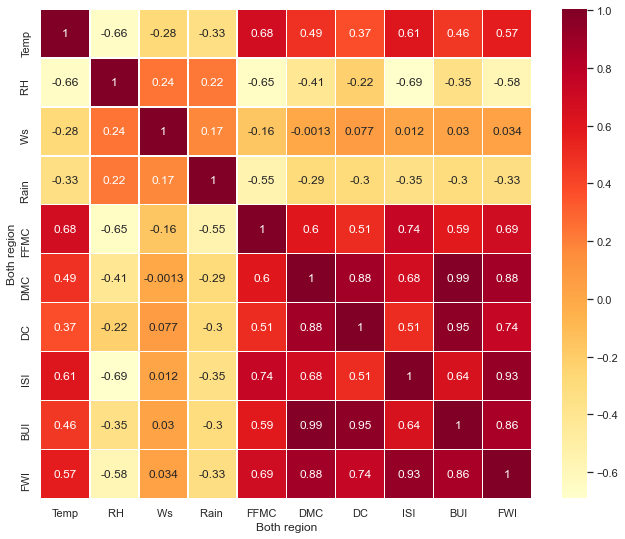
\includegraphics[scale=0.50]{Figures/CorrelationMap2.png}
    \caption{Heat map of the correlation coefficients for all 10 attributes of the both regions.}
    \label{fig:heatmap}
\end{figure}

\subsection{Classification from given meteorological inputs}

Before performing a Principal Component Analysis (PCA), the distribution of the output class "fire"/"not fire" can be depicted for the different meteorological inputs. This pre-analysis gives an estimation of the incidence of each of those inputs on the occurrence of fires. A general overview for the entire data set is given by the scatter plots in \autoref{fig:DataVisialization}. Also, scatter plots between meteorological attributes are depicted separately for both regions in \autoref{fig:scatter_comparison}. 

\begin{figure} [H]
    \centering
    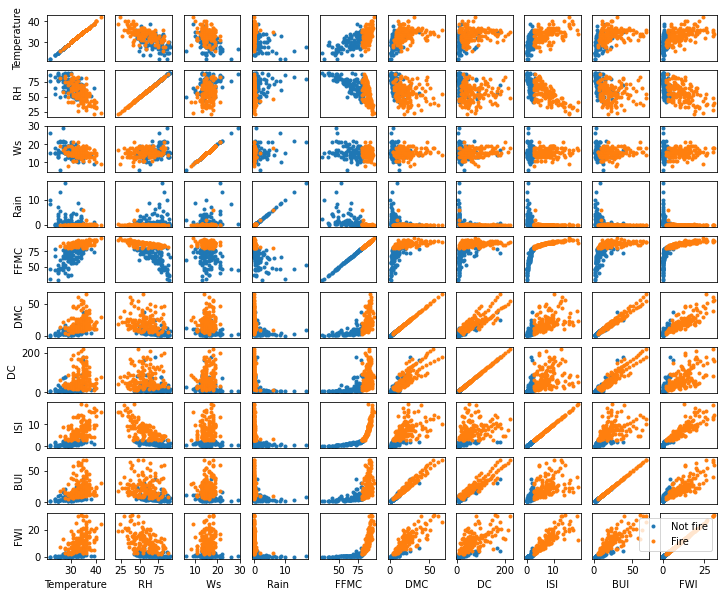
\includegraphics[scale=0.5]{Figures/DataVisualization.png}
    \caption{Scatter plots between the different 10 attributes for both regions.}
    \label{fig:DataVisialization}
\end{figure} 

\begin{figure}[H]
    \centering
    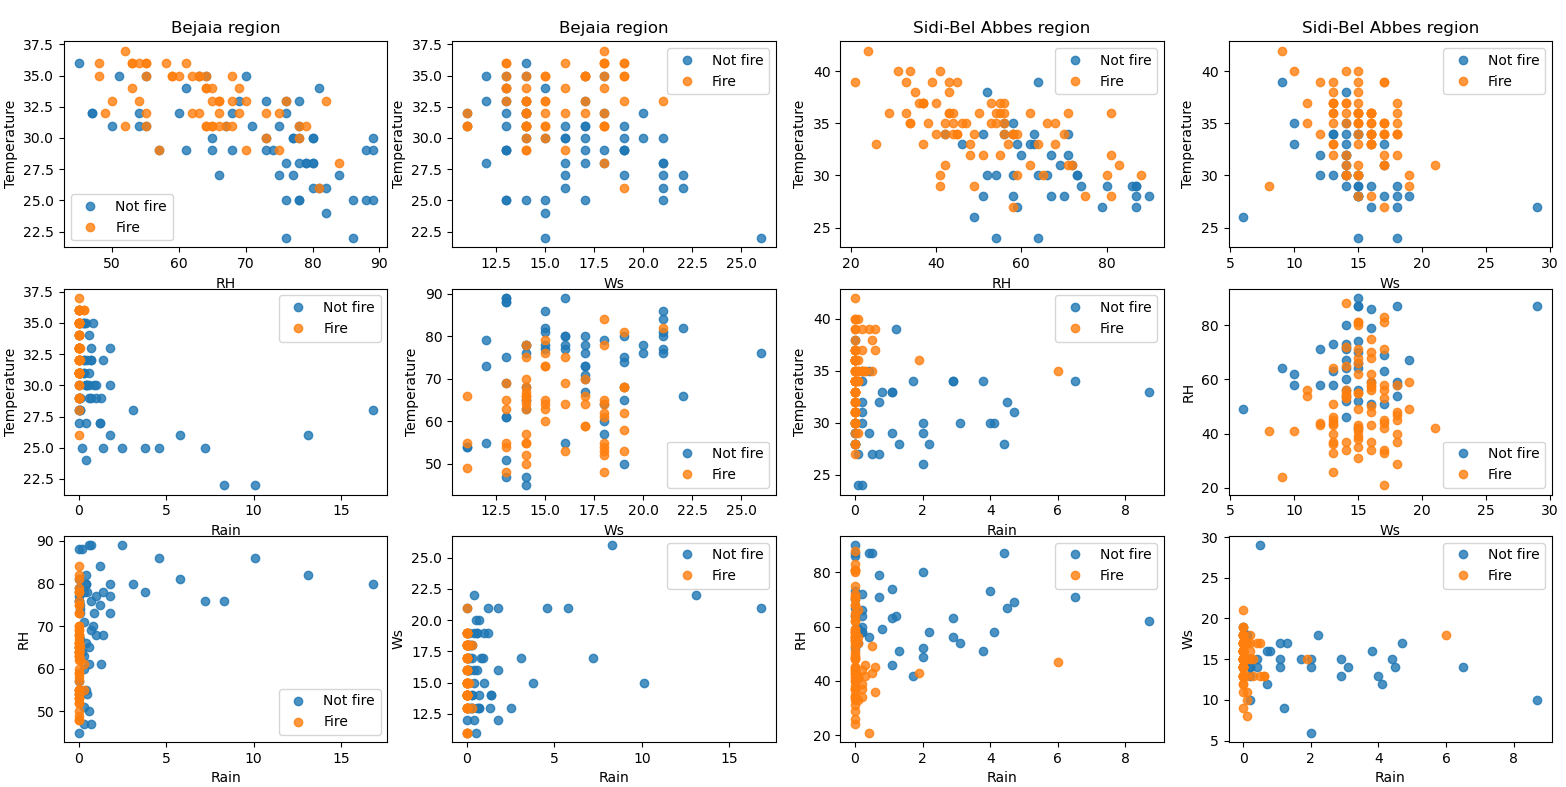
\includegraphics[width=\textwidth,height=\textheight,keepaspectratio]{Figures/compare_meteo_data.png}
    \caption{Comparison between Scatter plots of meteorological attributes for both regions}
    \label{fig:scatter_comparison}
\end{figure}

From \autoref{fig:scatter_comparison}, we can clearly see the existence of a correlation between high temperature, low relative humidity and fires, and this applying to both regions. Moreover, no clear pattern appears between wind speed and fires, although we could have expected, accordingly with the FWI system (see \autoref{fig:FWIstructure}), that higher wind speeds foster the propagation of fires. This can be partially explained by the fact that higher wind speeds are also associated with higher relative humidity and higher precipitations as revealed by the correlation study in \autoref{correlationStudy}. The direct effect of higher wind speeds in favor of fires would therefore be compensated by wetter conditions. Regarding precipitations, the scatters show that nearly all fires occur in their absence. Here it is worth mentioning that the original study \cite{article} does not include precipitation in its algorithm considering it an irrelevant parameter for the employed Decision Tree. We will however keep this attribute in the present analysis as it seems a priori to play a key role in the ignition of fires. Finally, \autoref{fig:FWIscatter} reveals the capacity of the two Fire Weather Index indices (FWI and FFMC) to determine quite efficiently the presence of fires. The occurrence of fires corresponds indeed to high values of FWI and FFMC.

\begin{figure} [H]
    \centering
    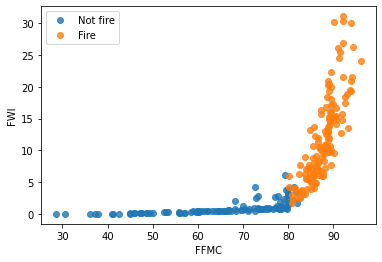
\includegraphics[scale=0.65]{Figures/FFMCVsFWI_Fires.png}
    \caption{Scatter plot of FFMC versus FWI for all the observations in both regions and identification of occurrences of fires.}
    \label{fig:FWIscatter}
\end{figure}

\subsection{Principal Component Analysis}

\subsubsection{General method}

The Principal Component Analysis (PCA) provides an insight in the relative variation of the attributes. It also enables to dimensionally reduce the data, which leads to decrease computational cost of Machine Learning algorithms as well as avoiding overfitting and redundancy in some circumstances.

Before computing the principal components, the observations matrix has been normalized by subtracting the mean and standardized by dividing by standard deviation. The necessity to divide by the standard deviation stems from the important variation of the standard deviations of different attributes (see \autoref{table:statistics_bejaia} and \autoref{table:statistics_bejaia}). We therefore compute:

\begin{equation}
    \widetilde{x}_{ij} = \frac{x_{ij} - m_j}{s_j}
\end{equation}
\noindent where $m_j$ and $s_j$ are the mean and the standard deviation of the attribute $j$.


\vspace{5mm}

Then, Singular Value Decomposition (SVD) has been used in order to compute the 10 eigenvectors and the 10 eigenvalues corresponding to the principal component directions.

\begin{equation}
    \boldsymbol{U \Sigma V^T} = \boldsymbol{X}
\end{equation}

\noindent where $\boldsymbol{V^T}$ contains in its columns the coordinates of the principal components (eigenvectors) and $\boldsymbol{\Sigma}$ has the singular values (or eigenvalues) in its diagonal. The variance explained is then calculated and depicted in \autoref{fig:Varexplained}.

\begin{equation}
    Variance\: explained = \frac{\sum_{i=1}^n \sigma_i^2}{\sum_{i=1}^{10} \sigma_i^2}
\end{equation}

\noindent with $\sigma_i$ the singular value of the $i^{th}$ principal component and $n$ the number of the components which is being considered. 

\begin{figure} [H]
    \centering
    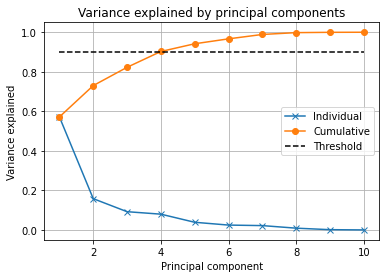
\includegraphics[scale=0.5]{Figures/VarianceExplained.png}
    \caption{Variance explained of the attributes divided by their standard deviation}
    \label{fig:Varexplained}
\end{figure}

\subsubsection{Effect of the standardization}

The following scatter plots (\autoref{fig:PC1PC2withStd} and \autoref{fig:PC1PC2WithoutStd}) present the distribution of all the observations along the two first principal components both before and after standardizing the data. We notice that the separation of the classes and the spread of the data are enhanced by standardizing the data. Also, in \autoref{fig:VarexplainedWithoutStd} we see that, if no standardization is applied, 90\% of the variance is explained just by the first component. This must be due to the fact that some attributes are over-represented and other under-represented in the variance of the data. Hence, this representation without standardization would result in a significant loss of information.

\begin{figure} [H]
    \centering
    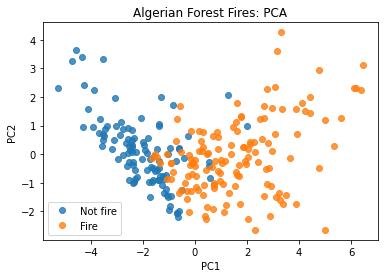
\includegraphics[scale=0.5]{Figures/PC1VsPC2_withStandardizing.png}
    \caption{PC1 and PC2 with division of the attributes by their standard deviation.}
    \label{fig:PC1PC2withStd}
\end{figure}

\begin{figure} [H]
    \centering
    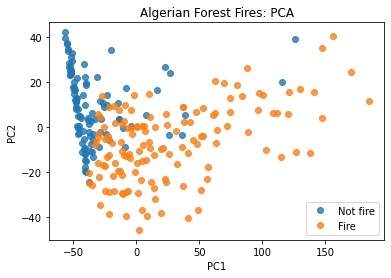
\includegraphics[scale=0.5]{Figures/PC1VsPC2_withoutStandardizing.png}
    \caption{PC1 and PC2 without division of the attributes by their standard deviation.}
    \label{fig:PC1PC2WithoutStd}
\end{figure}

\begin{figure} [H]
    \centering
    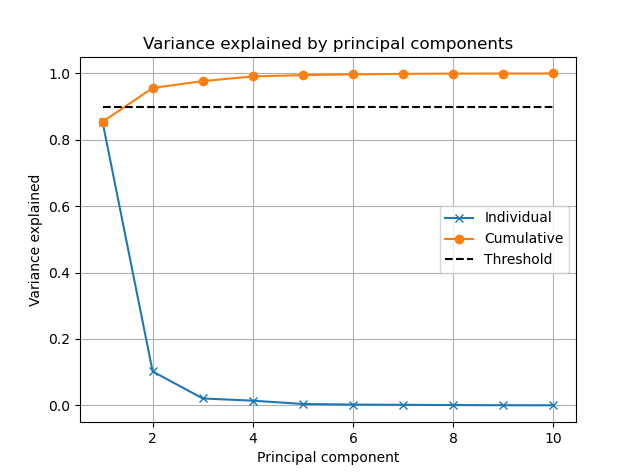
\includegraphics[scale=0.5]{Figures/variance_explained_no_standardization.png}
    \caption{Variance explained of the 10 attributes without the division by their standard deviation}
    \label{fig:VarexplainedWithoutStd}
\end{figure}

\subsubsection{PCA analysis for the whole data set}

In order to obtain a better representation of the attributes, it is important to find on which subspace it is better to project the data. Therefore, from the variance explained plot in \autoref{fig:Varexplained}, we see that the four first principal components are sufficient to explain more than 90\% of the variance of the data. 

Those four components should then be retained for further Machine Learning process. In \autoref{fig:PCAcoeff1} and \autoref{fig:PCAcoeff2}, the coefficients of the 4 principal components are represented for all 10 attributes of the data set in both regions separately. This enables to characterize the composition of the 4 principal directions. Especially, we see that the first principal direction, accounting for roughly 57\% of the variance, is composed of the temperature and all the indices FFMC to FWI and the opposite of the relative humidity and of the rain. This is consistent with the correlation analysis realized previously: FWI is higher for higher temperature and lower rain and relative humidity. The second direction corresponds to 15.8\% of the variance, the third 9.3\% and the fourth 8.0\%. Those last three components are therefore significantly less important to understand the variation of attributes in the data. They correspond to secondary patterns such as, for the second component in Bejaia region, the negative correlation between temperature on one side, and relative humidity, wind speed and rain on the other side. We also note that the patterns are different between the two regions for those "secondary" components. Those secondary patterns are nevertheless essential to account for a total of more than 90\% of the variance.

The scatter plot in \autoref{fig:PC1PC2withStd} shows the capacity of the two first components to classify the events between "fire" and "not fire". However, when considering only those two directions, the classification seems to be slightly less neat than when using FFMC and FWI (see \autoref{fig:FWIscatter}). This could be further analyse comparing the Machine Learning algorithm results working from FFMC and FWI or from the four first principal component.





\subsubsection{PCA for Bejaia region}
The first four principal components for the Bejaia region are:
\begin{equation*}
    v1 = 
        \begin{bsmallmatrix}
            \
        0.31\\
        -0.25\\
        -0.04\\
        -0.19\\
        0.34\\
        0.36\\
        0.35\\
        0.37\\
        0.36\\
        0.38
           
        \end{bsmallmatrix}, \hspace{7pt}
    v2 = 
        \begin{bsmallmatrix}
           \
                -0.27\\
                0.35\\
                0.55\\
                0.41\\
                -0.25\\
                0.26\\
                0.28\\
                0.00\\
                0.27\\
                0.17
            
        \end{bsmallmatrix}, \hspace{7pt}
    v3 = 
        \begin{bsmallmatrix}
           \
                0.20\\
                -0.57\\
                0.48\\
                0.44\\
                0.12\\
                -0.20\\
                -0.21\\
                0.19\\
                -0.20\\
                0.02
            
        \end{bsmallmatrix}, \hspace{7pt}
    v4 = 
        \begin{bsmallmatrix}
           \
                -0.06\\
                -0.18\\
                -0.66\\
                0.66\\
                -0.18\\
                0.13\\
                0.03\\
                0.01\\
                0.09\\
                0.10
          
        \end{bsmallmatrix}.
                  
\end{equation*}



\begin{figure} [H]
    \centering
    \textbf{Bejaia Region}\par\medskip
    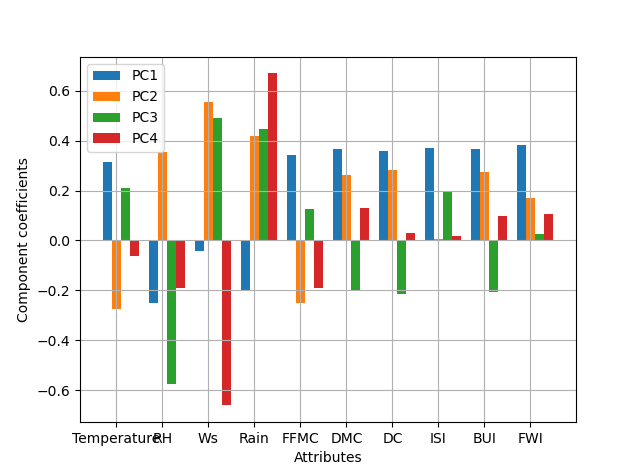
\includegraphics[scale=0.5]{Figures/PC_components_coeff_first_region.png}
    \caption{PCA component coefficients for the 10 attributes of Bejaia region.}
    \label{fig:PCAcoeff1}
\end{figure}

\autoref{fig:PCAcoeff1} shows that the 4th principal component has the largest coefficient for the rain and Ws attributes from the Bejaia region, therefore a projection that shows an acceptable division between the Fire and Not fire class, might indicate a correlation of the presence of fires with a low amount of rain and high amount of wind speed. 
The projection over the different principal components are shown in \autoref{first_region_proj}.
\begin{figure}[H]
    \centering
    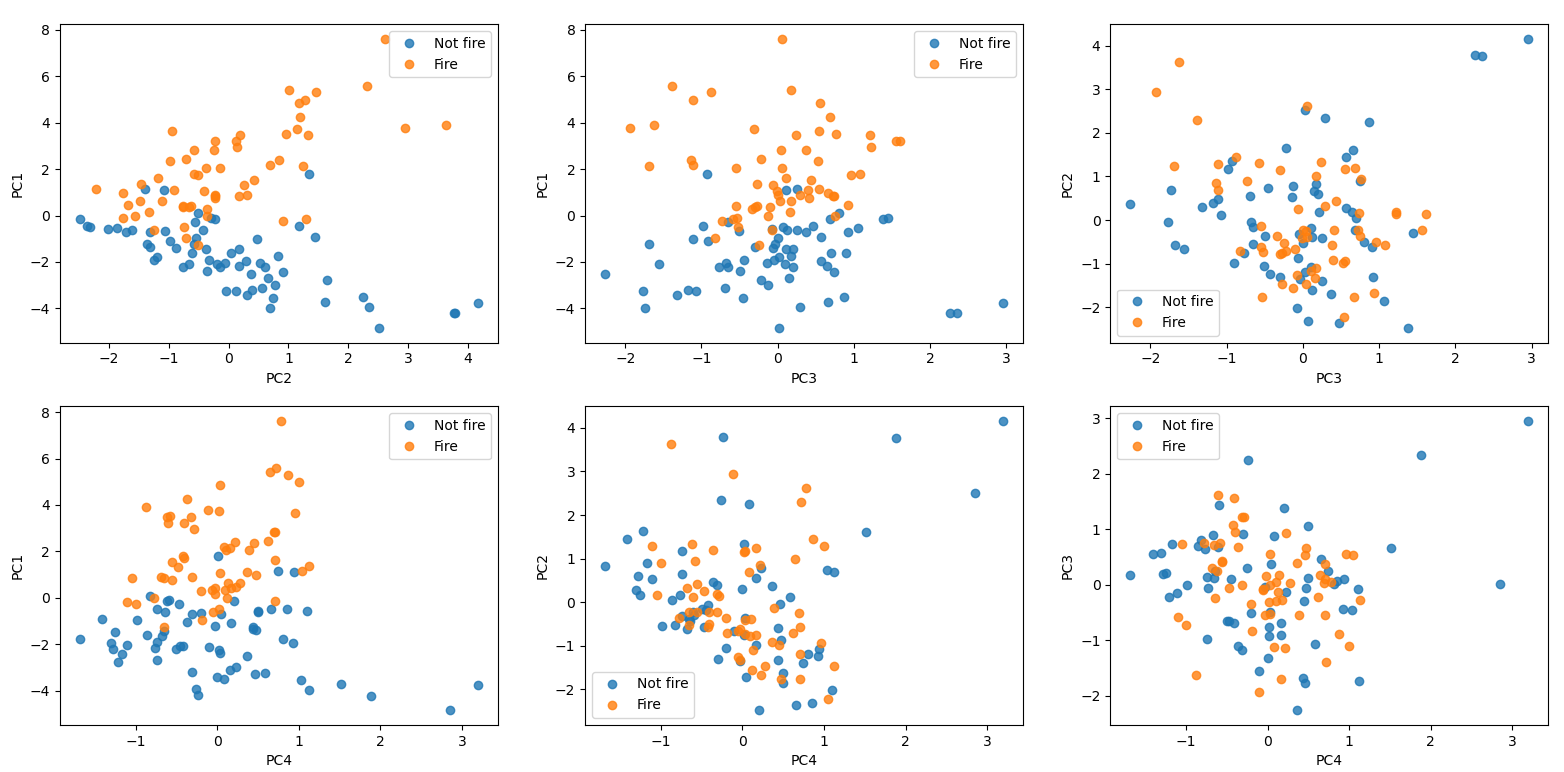
\includegraphics[width=\textwidth,height=\textheight,keepaspectratio]{Figures/projection PC first region.png}
    \caption{Projection of data over the principal components for the Bejaia region}
    \label{first_region_proj}
\end{figure}

From \autoref{first_region_proj} it is possible to see that the projection on PC2, PC3 and PC4 don't show an acceptable separation between the two classes, therefore no conclusion regarding the correlation between fires and meteorological conditions can be drawn from those components. Nevertheless the projection over PC1 shows a nice separation between the 'Fire' and 'Not fire' classes, hence, since the Fire observations have a positive projection over PC1, they can be correlated to high values for the Fire Weather Indexes (FFMC,DMC,DC,ISI,BUI,FWI), low amount of rain and relative humidity and high temperature, based on the coefficients shown in \autoref{fig:PCAcoeff1}







\subsubsection{PCA for Sidi-Bel Abbes region}


The first four principal components for the Sidi-Bel Abbes region are:
\begin{equation*}
    v1 = 
        \begin{bsmallmatrix}
            \
            0.25\\
            -0.27\\
            -0.008\\
            -0.20\\
            0.34\\
            0.37\\
            0.33\\
            0.36\\
            0.37\\
            0.40
            
        \end{bsmallmatrix}, \hspace{7pt}
    v2 = 
        \begin{bsmallmatrix}
        \
                0.48\\
                -0.46\\
                -0.46\\
                0.19\\
                0.18\\
                -0.24\\
                -0.32\\
                0.13\\
                -0.27\\
                -0.04
           
        \end{bsmallmatrix}, \hspace{7pt}
    v3 = 
        \begin{bsmallmatrix}
           \
                -0.07\\
                -0.14\\
                0.62\\
                -0.4\\
                0.22\\
                -0.26\\
                -0.34\\
                0.29\\
                -0.28\\
                0.05
            
        \end{bsmallmatrix}, \hspace{7pt}
    v4 = 
        \begin{bsmallmatrix}
            \
                0.036\\
                -0.21\\
                0.48\\
                0.78\\
                -0.2\\
                0.06\\
                -0.02\\
                0.16\\
                0.04\\
                0.15
           
        \end{bsmallmatrix}.
                  
\end{equation*}

\begin{figure} [H]
    \centering
    \textbf{Sidi-Bel Abbes region}\par\medskip
    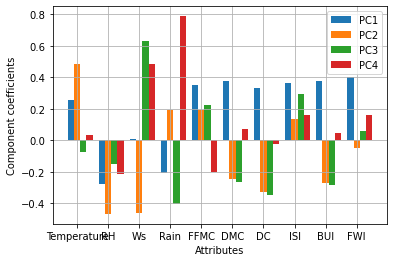
\includegraphics[scale=0.5]{Figures/PC_components_coeff_second_region.png}
    \caption{PCA component coefficients for the 10 attributes.}
    \label{fig:PCAcoeff2}
\end{figure}

\autoref{fig:PCAcoeff2} shows that PC4 and PC3 have the largest coefficients for rain and wind speed respectively.

The projections on the different principal components are shown in \autoref{second_region_proj}



\begin{figure}[H]
    \centering
    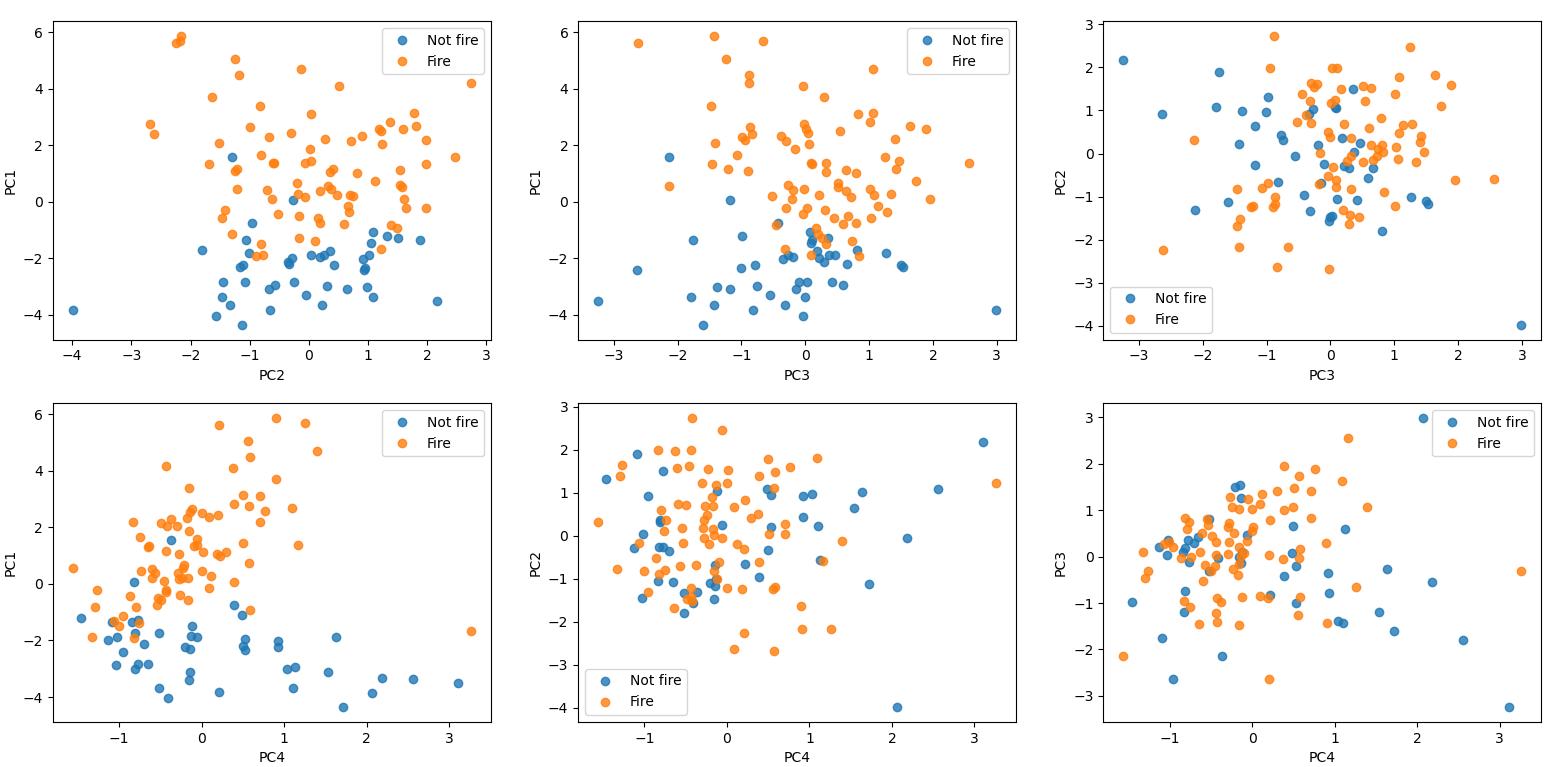
\includegraphics[width=\textwidth,height=\textheight,keepaspectratio]{Figures/projection PC second region.png}
    \caption{Projection of data over the 3rd and 4th principal components for Sidi-Bel Abbes region}
    \label{second_region_proj}
\end{figure}

As for the case of Bejaia region, the projection on PC1 shows a separation of the two classes and the projection of Fire data leads to a positive projection on PC1, which correspond to high values of the Fire Weather Indexes, low amount of rain and relative humidity and high temperature.

In conclusion, from the projection of the data over its own principal components, only the projection on PC1 shows a acceptable separation between the two classes, which is understandable since the PC1 accounts for roughly 57\% of the total variance.


Nevertheless, it must be noticed how the relation between the coefficients of PC2, PC3 and PC4 and the meteorological attributes are very different between the two regions, which leads to different projections for the two region on these principal components.
This could be a consequence of the different climate found in the two regions, as analysed in \autoref{section:data visualisation}, where it is shown that the Sidi-bel Abbès region has a more arid climate in comparison to the Bejaia region, where higher amount of precipitation and lower temperatures were recorded.














\section{Perspectives of Machine Learning study}
\label{Perspectives}

Considering the studied data set and its principal characteristics revealed in the present analysis, it would be possible to carry several tasks with different Machine Learning algorithms. 

The more obvious task and the most straight to the point, would be to predict the presence of fires based on the knowledge of the meteorological characteristics. In this approach, we would assume that the FWI indices are also known variables, provided that the meteorological characteristics yield directly the values of all the indices via a deterministic calculation scheme (detailed in Van Wagner, 1987, \cite{FWI_Wagner}). This task would be the first to achieve in a realistic situation where, as in the reference study (\cite{article}), the objective is to warn the propagation of fires at some geographical location where meteorological measure instruments are installed.

A second classification task would be also to predict the fires but this time without providing the FWI indices. We will employ the existed data (without FWI attribute) with fire/not fire label to train a classification model, and then use this model to predict if fire disaster would happen when data in a specific day are provided. The performance of this algorithm, compared with the first one, would provide an insight on the importance of using the FWI indices, and would answer the question of knowing if a Machine Learning algorithm could do as well as the FWI indices in determining the presence of fires. We saw indeed in the present report that the classes fire/not fire were most correctly distinguished when considering the FFMC and FWI indices.

Related to the later problematic, would be a third task, namely of regression, which would answer the question: how would perform a Machine Learning algorithm in determining the FWI index which is normally obtained through the FWI system described by E.C. Van Wagner \cite{FWI_Wagner}? The proposal regression would take into account the four meteorological components as inputs and would return the predicted FWI index as output. Finally, we would evaluate this regression model in the light of an error analysis, where the root mean square errors between the actual FWI and the predicted FWI would be calculated.

Another problematic would be to determine if the constructed algorithms are independent of the region. If we notice some significant variations in the results of the algorithm between the two regions it would indicate that some determinant parameters dependant on the region are not taken into account (eg. type of vegetation). This analysis would imply to train for instance two algorithms, one on each region and then apply them both to the same region for comparison. Furthermore, at the end of this analysis, a final step would be to build a more general model to predict forest fires situation in an other region after the attributes of the other region are given. 

\begin{thebibliography}{}
\bibitem{article} Faroudja Abid, Nouma Izeboudjen, 06 February 2020, \textit{Predicting Forest Fire in Algeria Using Data Mining Techniques: Case Study of the Decision Tree Algorithm}

\bibitem{FWI_Wagner} C.E Van Wagner, 1987, \textit{Development and Structure of the Canadian Forest Fire Weather Index System}

\end{thebibliography}

\end{document}

